\usetikzlibrary{shapes.geometric}
\usetikzlibrary{angles}
\definecolor{myblue}{rgb}{0.067,0.529,0.871}
\definecolor{mypurple}{rgb}{0.859,0.071,0.525}
\definecolor{myred}{rgb}{1.0, 0.13, 0.32}
\definecolor{mygreen}{rgb}{0.01, 0.75, 0.24}
\def\PolyRadius{2cm}
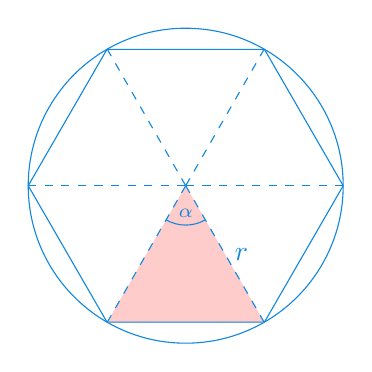
\begin{tikzpicture}[draw=myblue, text=myblue	]
\draw (0,0) circle (2);
\coordinate (A) at (-1,-1.74);
\coordinate (B) at (0,0);
\coordinate (C) at (1,-1.74);
\fill[fill=red!20] (0,0) -- (-1,-1.74) -- (1, -1.74) -- (0,0);
\node[regular polygon,draw,regular polygon sides = 6,minimum size=2*\PolyRadius] at (0,0) {};
\draw pic[draw,angle radius=0.5cm]{angle=A--B--C};
\node at (0,-0.35) {\scriptsize $\alpha$};
\draw [dashed] (0,0) -- (2,0);
\draw [dashed] (0,0) -- (-2,0);
\draw [dashed] (0,0) -- (1,1.74);
\draw [dashed] (0,0) -- (-1,1.74);
\draw [dashed] (0,0) -- (-1,-1.74);
\draw [dashed] (0,0) -- (1,-1.74) node[right, midway] {$r$};
\end{tikzpicture}
